\documentclass[10pt]{article}
\usepackage[margin=0.8in]{geometry}
\usepackage[T1]{fontenc}
\usepackage{lmodern}
\usepackage{microtype}
\usepackage{amsmath}
\usepackage{amsthm}
\usepackage{booktabs}
\usepackage{graphicx}
\usepackage{float}
\usepackage{hyperref}
\usepackage{xcolor}
\graphicspath{{./}}
\hypersetup{colorlinks=true,linkcolor=blue,citecolor=blue,urlcolor=blue}

\newtheorem{definition}{Definition}
\newtheorem{lemma}{Lemma}

\newcommand{\poolocc}{\mathit{pool\_occ}}

\title{Dimension Pool: Deadlock-Safe Buffer Pooling Across Opposing
Inports on a 3D Torus\\
\large Lab 4 Project Report --- Topic 2: Flow Control}
\author{}
\date{\today}

\begin{document}
\maketitle

\begin{abstract}
Classical virtual-channel (VC) allocation statically splits each router's
buffers per inport, so when traffic through a dimension is momentarily
one-sided --- the common case on a torus --- the cold direction's VCs sit
idle while the hot direction head-blocks. This report presents
\emph{Dimension Pool} (DP), a flow-control mechanism in which the two
opposing inports of each dimension ($E{+}W$, $N{+}S$, $U{+}D$) share their
pooled VCs under a joint occupancy cap $S$, letting a hot direction borrow
budget the cold direction is not using --- without relocating any packet
and without touching the deadlock-freedom substrate. DP composes with two
independently deadlock-free baselines on the same 4$\times$4$\times$4
Garnet Torus3D substrate: dimension-order routing protected by the
Critical Bubble Scheme (DP-CBS) and minimal adaptive routing with escape
VCs (DP-ESC). Under an equal-usable-storage methodology (a DP
configuration is compared against a plain baseline with the same usable
slots per dimension pair), DP-ESC gains \textbf{+21--31\%} peak stable
throughput on all five synthetic patterns at budget $C{=}6$, and DP-CBS
gains \textbf{+20.9\%} on xopposite at $C{=}6$. All 1006 runs, including
six 200\,000-cycle saturation probes, are deadlock-free. We also report
the mechanism's costs honestly: the shared cap loses up to $-32.6\%$ at
equal VC count under two-sided load, DP-CBS turns slightly negative
($-2.7\%$) once buffers are plentiful ($C{=}8$), and gains on symmetric
uniform-random traffic are near zero --- pooling pays exactly where demand
between directions is imbalanced.
\end{abstract}

\section{Introduction}

On a torus, the $+d$ and $-d$ directions of a dimension are rarely equally
loaded at a given router and moment: adversarial patterns (xopposite,
tornado) are strictly one-sided per ring, and even balanced patterns are
one-sided \emph{locally} over short windows. Yet the standard Garnet
buffer organization dedicates every VC to one inport, i.e.\ to one
direction. The result is a structural inefficiency: the hot side
saturates on its private slots while the opposite side's slots are
provably idle.

Dimension Pool (DP) removes this split at the accounting level. The
pooled VCs of the two opposing inports form one budget, admission into any
pooled VC requires the \emph{joint} occupancy to stay below a cap $S$, and
nothing else changes: no packet ever moves between buffers, the datapath
and crossbar are untouched, and deadlock freedom is delegated to a
substrate that is never pooled. Highlights:

\begin{itemize}
  \item \textbf{A new flow-control primitive.} DP is neither a VC
    reassignment scheme nor a shared physical buffer (DAMQ): it is a
    counter-only occupancy budget spanning two inports, cheap enough to
    sit in the allocator's existing credit checks.
  \item \textbf{Two deadlock-safety compositions.} DP-CBS runs the
    Critical Bubble Scheme~\cite{chen2011} verbatim on a private
    dedicated tranche (a ``depth-domain'' instance of Duato's
    argument~\cite{duato1993}); DP-ESC exempts escape
    VCs~\cite{dally1987,duato1993} from the pool so Duato's theorem
    applies unchanged. In both, the pool is a pure performance resource:
    pooled admission may fail at any time without risking deadlock.
  \item \textbf{An equal-usable-storage methodology.} Every DP
    configuration is compared against a plain baseline with the same
    usable slots per dimension pair, so measured wins come from pooling
    flexibility, not extra buffers. Claims are further stress-tested by
    cap-falsification reruns ($S{=}1$) and a bit-identical baseline-purity
    check.
  \item \textbf{Honest accounting of costs.} We report where DP loses
    (equal-VC two-sided load, buffer-rich regimes) and where it is
    neutral (uniform random), alongside the +21--31\% headline gains.
\end{itemize}

This report covers Topic 2 (flow control). The Torus3D topology, the
adaptive routing algorithm with Mesh3D-routed escape VCs, and the plain
CBS implementation that DP builds on are covered in the companion Topic 1
report; here they serve as \emph{baselines}.

\section{Substrate and Baselines}
\label{sec:baselines}

\subsection{Common substrate}

All experiments run on gem5 Garnet (standalone), 4$\times$4$\times$4
Torus3D (64 nodes), synthetic traffic on control vnet~0 with single-flit
packets. Control VCs hold one packet each
(\texttt{buffers\_per\_ctrl\_vc}~=~1), so a buffer \emph{slot}, a VC, and
a packet-in-flight coincide; DP bookkeeping is pure counting.

\subsection{Baseline family A: DOR + Critical Bubble Scheme}

Deterministic dimension-order routing (DOR) on a torus deadlocks on the
wrap-around rings. The Critical Bubble Scheme (CBS)~\cite{chen2011}
restores safety without reserving VC classes: one buffer slot per
directed ring is marked \emph{critical} and may only be consumed by
in-transit packets, never by injection, so every ring always retains a
bubble and can drain. Family A baselines (A1, A3 in
Table~\ref{tab:configs}) run DOR + CBS with 3 and 4 VCs per inport.

\subsection{Baseline family B: minimal adaptive routing + escape VCs}

Family B uses the Topic 1 adaptive router: minimal-quadrant adaptive
routing over the torus wrap links, with the last VC of each inport
reserved as an escape channel routed by deadlock-free (acyclic-CDG)
Mesh3D XYZ routing. By Duato's theorem~\cite{duato1993}, a packet blocked
on adaptive VCs can always eventually take the escape path, so the
adaptive tranche may be arbitrarily congested. Baselines B1, B3, B5 run
this design with 2, 3, 4 VCs per inport.

\section{Design: the Dimension Pool}
\label{sec:design}

\subsection{Pool, cap, and tranches}

For each router, dimension $d$, and control vnet, define
\begin{equation}
  \poolocc(R, d, v) \;=\; \mathit{occ}(\text{inport } {+}d) +
  \mathit{occ}(\text{inport } {-}d),
\end{equation}
where $\mathit{occ}$ counts packets currently holding a \emph{pooled} VC
at that inport, from allocation grant until the freeing credit returns.
Admission into any pooled VC requires
\begin{equation}
  \poolocc < S \qquad (S = \texttt{--dp-shared-cap}).
\end{equation}
There is no ``enable event'' and no slot transfer: borrowing is emergent.
When one side is idle it contributes $\approx 0$ to $\poolocc$, so the hot
side can occupy up to all $S$ units of the pair budget; under two-sided
load the two inports compete for the same budget.

VCs are partitioned into tranches that are \emph{ID-pegged} (fixed at
configuration time, a property of the VC id --- count-based accounting
would break the CBS bubble invariant, which needs the identity of the
critical slot to be stable):

\begin{itemize}
  \item \textbf{DP-CBS} (on family A): VC ids $[0, r)$ are a
    \emph{dedicated} tranche private to the inport ($r{=}2$ throughout);
    ids $[r, V)$ are pooled.
  \item \textbf{DP-ESC} (on family B): the adaptive window $[0, V-1)$ is
    pooled; the escape VC is \emph{exempt} --- never counted in
    $\poolocc$, never denied by the cap.
\end{itemize}

When both a pooled and a dedicated VC are free, the allocator prefers the
pooled one: spending shared budget before private reserve maximizes
bubble mobility in the dedicated sub-ring. (The design mirrors pooled
liquidity with a private per-direction reserve in payment-channel
networks; the reserve guarantees progress, the pool provides the
flexibility.)

\subsection{Admission and retry semantics}

The pool check is a \emph{pre-flight} credit-style test: a packet that
fails admission never leaves its upstream VC; there is no NACK, drop, or
retransmission. Switch allocation re-arbitrates every cycle, so a denied
packet simply retries. The two variants differ in where the primary
check sits:

\begin{itemize}
  \item \textbf{DP-ESC}: the primary check is a candidate filter inside
    the adaptive route computation --- an outport whose downstream pool is
    full is skipped exactly like an outport with zero free credits, so
    the packet either picks another minimal adaptive direction or falls
    through to the escape VC via the existing machinery. A belt check in
    \texttt{send\_allowed} covers the race where the pool fills between
    route computation and switch allocation. This placement preserves
    Duato's premise: a packet waiting on adaptive resources always still
    has the escape path available.
  \item \textbf{DP-CBS}: DOR fixes the outport, so the check sits in the
    switch allocator's admission rule; on failure the packet waits for,
    or falls back to, the dedicated tranche under normal CBS entry rules.
\end{itemize}

\subsection{Deadlock safety}
\label{sec:safety}

DP only ever \emph{restricts} admission to pooled slots and changes no
routes, but pooling alone is not safe. Suppose one kept only the cap rule
with no discipline inside the private slots: on a single ring under DOR,
every node injecting in one direction can fill \emph{all} private and
pooled slots with packets each waiting for the next hop --- the cap is
respected at every router, yet the ring holds no free slot and deadlocks.
A cap bounds \emph{how many} slots each side holds; deadlock freedom
needs an invariant about \emph{which} slot stays free. DP therefore
composes with a substrate that provides exactly that invariant:

\textbf{DP-CBS: depth-domain Duato.} The dedicated window $[0,r)$ runs
CBS verbatim as a private sub-ring of depth $r$: ring entry toward a
marked inport requires two free dedicated slots, and in-ring transit may
fill the last free dedicated slot only if the mover itself resides in a
dedicated VC --- otherwise a packet sitting in a pooled VC could consume
the bubble while returning its own slot to the pool, where the opposite
direction may claim it, and the sub-ring would lose its bubble
permanently. The pooled window is the ``adaptive layer'' of a Duato
construction, transplanted from VC class to buffer depth: it may be
arbitrarily congested because every packet in it is also eligible for the
dedicated (escape) layer at every hop.

\textbf{DP-ESC: Duato verbatim.} Escape VCs are exempt from the pool, so
the escape network's acyclic channel-dependency graph is untouched and
Duato's theorem applies unchanged.

\textbf{Conservative accounting.} $\poolocc$ is incremented at
switch-allocation grant (a reservation, before the flit moves) and
decremented when the freeing credit returns, so occupancy spans
grant\,$\to$\,credit-return and slightly overestimates instantaneous
buffer occupancy. Because the pool is never in the safety path, this
staleness can only cost throughput, never correctness. Same-cycle
over-admission is excluded by gem5's sequential router wakeup together
with a configuration guard requiring all torus dimensions $\ge 3$ (a
size-2 dimension would let both outports of one router feed the same
downstream pool in one cycle).

\subsection{Hardware cost}

DP's state is three $\lceil \log_2(S{+}1) \rceil$-bit counters per router
per control vnet (one per dimension pair) plus an adder and comparator in
the allocator --- negligible next to the buffers themselves. The real new
item is \emph{wiring}: the joint occupancy of a downstream router's two
inports must be visible to two different upstream routers. In simulation
the registry is a zero-latency oracle; a hardware realization keeps the
counter at the downstream router and distributes a token-conserved
pool-credit sideband of roughly one wire per link per pooled vnet,
piggybacking on the existing credit channel. Because tranches are
ID-pegged, an implementation over-provisions VC ids (build $2\times$
pooled, use $\le S$) rather than porting a dual-ported shared SRAM ---
cheap for one-flit control slots. Datapath, crossbar, and pipeline are
untouched.

\section{Implementation}
\label{sec:impl}

DP is implemented in gem5 v23.0 Garnet behind \texttt{--enable-dp}
(default off; all baseline paths bit-identical when disabled, verified in
\S\ref{sec:validation}).

\begin{table}[H]
\centering
\small
\begin{tabular}{lp{0.62\textwidth}}
\toprule
File & Change \\
\midrule
\texttt{GarnetNetwork.py} / \texttt{Network.py} &
  \texttt{enable\_dp}, \texttt{dp\_reserve} ($r$), \texttt{dp\_shared\_cap}
  ($S$) parameters and CLI flags \\
\texttt{GarnetNetwork.hh/.cc} &
  occupancy registry \texttt{m\_dp\_shared\_occ[router][dir][vnet]},
  helpers, stats, config validation \\
\texttt{SwitchAllocator.cc} &
  DP-CBS admission rule, shared-first VC selection, grant-time
  increment, belt check \\
\texttt{OutputUnit.cc} &
  decrement on the returning \texttt{is\_free\_signal} credit \\
\texttt{RoutingUnit.cc} &
  pool-full candidate filter in the adaptive route computation (DP-ESC) \\
\bottomrule
\end{tabular}
\caption{Implementation map. Both bookkeeping sites address the
downstream buffer owner symmetrically.}
\label{tab:impl}
\end{table}

New statistics: \texttt{dp\_shared\_grants} (allocations landing in
pooled VCs) and \texttt{dp\_pool\_blocks} (admissions denied by the cap).
Configuration validation rejects unsupported operating points with
\texttt{fatal}: torus dimensions $\ge 3$, control vnets only, routing
algorithms 3/4 only, no wormhole, $S \in [1,\, 2\times\text{pooled per
inport}]$.

\section{Experiments}
\label{sec:experiments}

\subsection{Methodology: equal usable storage}

A DP configuration with $d$ dedicated VCs per inport and cap $S$ exposes
at most $C = 2d + S$ usable slots per dimension pair. Each DP mode is
compared against the plain baseline whose total storage per pair equals
that $C$ (Table~\ref{tab:configs}); DP carries more physical VC ids, but
their concentration on the hot inport is exactly the mechanism under
test, so wins cannot come from extra buffers.

\begin{table}[H]
\centering
\small
\begin{tabular}{llllc}
\toprule
Family & Baseline & DP configuration & DP parameters & $C$ \\
\midrule
A (DOR + CBS) & A1: vcs=3 & A2: vcs=4 & $r{=}2$, $S{=}2$ & 6 \\
              & A3: vcs=4 & A4: vcs=6 & $r{=}2$, $S{=}4$ & 8 \\
B (adaptive + escape) & B1: vcs=2 & B2: vcs=3 & $S{=}2$ & 4 \\
              & B3: vcs=3 & B4: vcs=5 & $S{=}4$ & 6 \\
              & B5: vcs=4 & B6: vcs=7 & $S{=}6$ & 8 \\
\bottomrule
\end{tabular}
\caption{Equal-usable-storage pairs. $C = 2\cdot\text{dedicated} + S$
usable slots per dimension pair.}
\label{tab:configs}
\end{table}

Sweep: five patterns (xopposite, tornado, transpose, neighbor, uniform
random) $\times$ 20 injection rates (0.05--1.00) $\times$ 10 modes = 1000
runs of 10\,000 cycles. Throughput is received packets/node/cycle; a
point is \emph{stable} when $\ge 90\%$ of offered load is accepted; the
offered-load ceiling of the harness is 0.5 packets/node/cycle.

\subsection{Results}

\begin{table}[H]
\centering
\small
\begin{tabular}{lccccc}
\toprule
Pair & xopposite & tornado & transpose & neighbor & uniform \\
\midrule
A, $C{=}6$ & \textbf{+20.9\%} & ceil & +1.4\% & ceil & $\ge$+2.6\% \\
A, $C{=}8$ & $-2.7\%$ & ceil & +1.3\% & ceil & ceil \\
B, $C{=}4$ & +37.1\% & +95.0\%$^{\dagger}$ & +87.5\%$^{\dagger}$ &
  +103.0\%$^{\dagger}$ & +95.7\%$^{\dagger}$ \\
B, $C{=}6$ & \textbf{+21.3\%} & $\ge$+31.0\% & $\ge$+29.2\% &
  $\ge$+24.9\% & $\ge$+28.5\% \\
B, $C{=}8$ & ceil & ceil & ceil & ceil & ceil \\
\bottomrule
\end{tabular}
\caption{Peak stable throughput gain of DP over its equal-storage
baseline. ``ceil'': both sides saturate the 0.5 injection ceiling (no
information). ``$\ge$'': the DP side is at the ceiling, so the gain is a
lower bound. $^{\dagger}$~budget-efficiency result, not a flow-control
gain --- see reading~2 below.}
\label{tab:gains}
\end{table}

\begin{figure}[tbp]
  \centering
  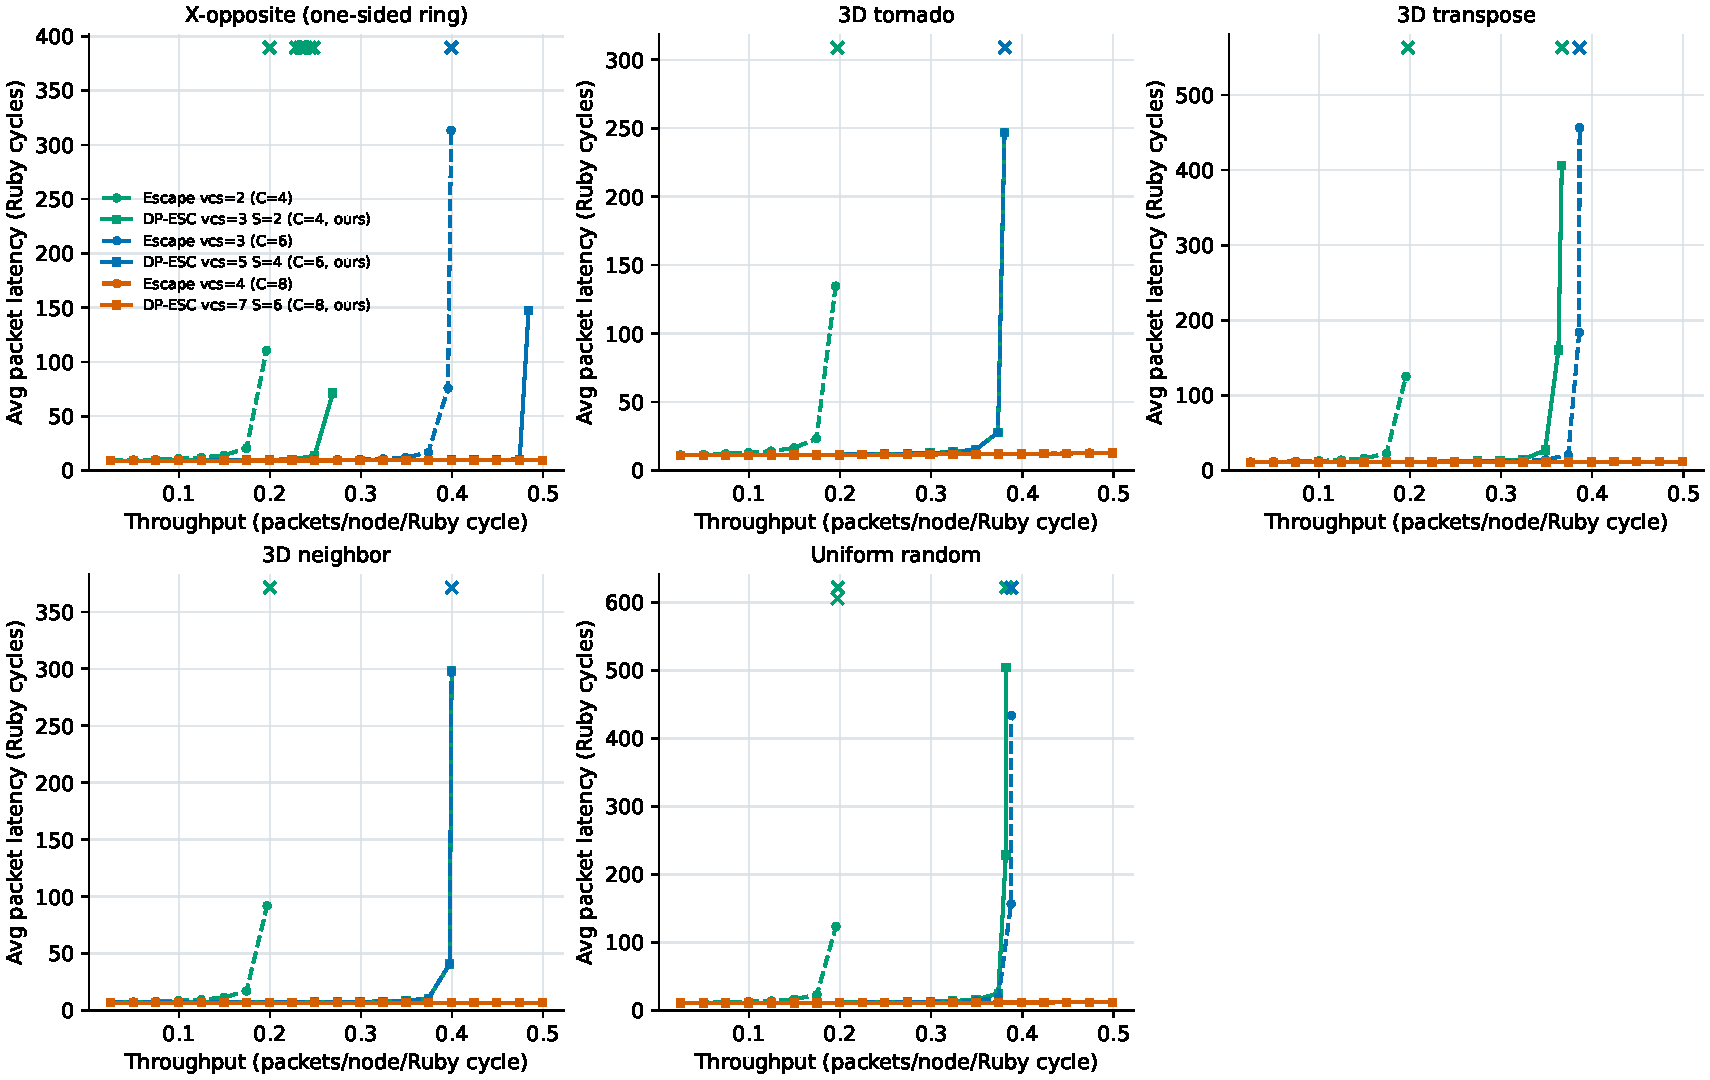
\includegraphics[width=0.82\textwidth]{latency_throughput_dp_b}
  \caption{Family B (adaptive + escape): latency--throughput curves per
  pattern. Solid/dashed lines are stable points; $\times$ markers are
  unstable points pinned to the top edge. DP curves extend the stable
  region to higher throughput at equal usable storage.}
  \label{fig:ltb}
\end{figure}

\begin{figure}[tbp]
  \centering
  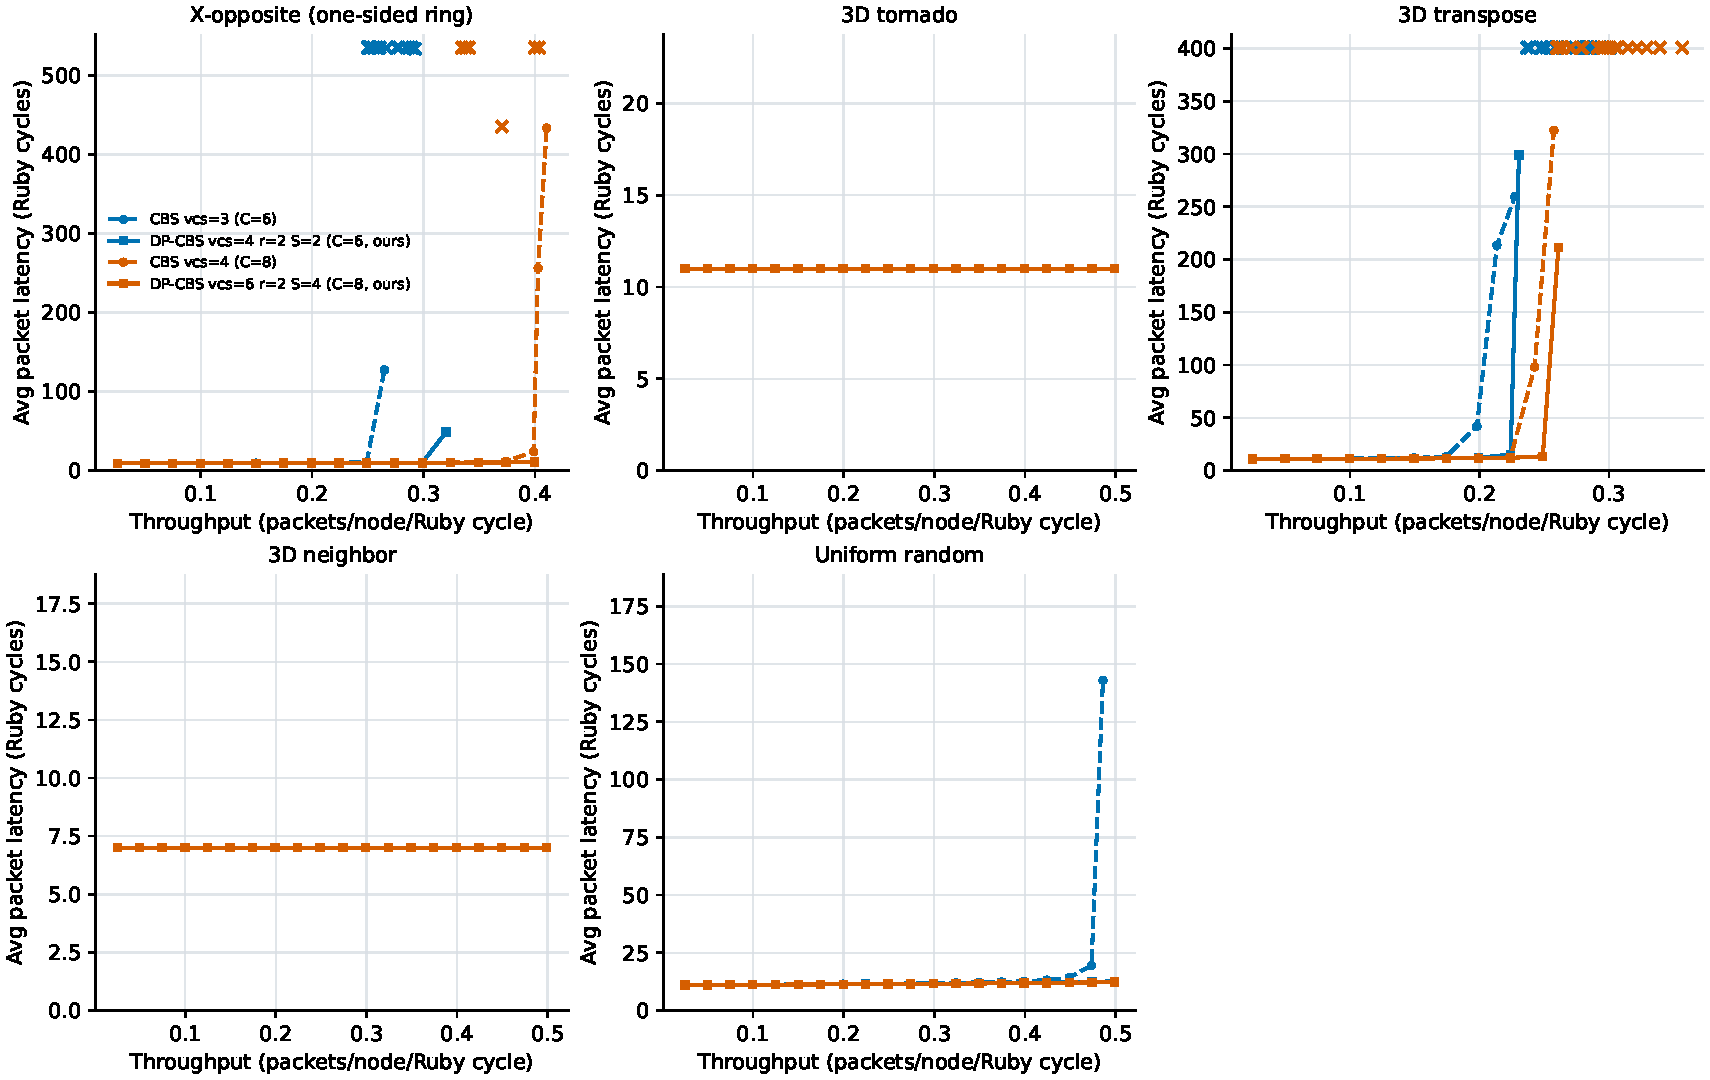
\includegraphics[width=0.82\textwidth]{latency_throughput_dp_a}
  \caption{Family A (DOR + CBS): latency--throughput curves per pattern.
  The xopposite panel shows the +20.9\% stable-region extension of A2
  over A1; at $C{=}8$ (A4 vs.\ A3) the ordering reverses.}
  \label{fig:lta}
\end{figure}

Four readings, in decreasing order of strength:

\begin{enumerate}
  \item \textbf{DP-ESC at $C{=}6$: +21--31\% on every pattern} (mostly
    lower bounds), including uniform random and including the one cell
    (xopposite) with no ceiling excuse. This is the headline claim.
  \item \textbf{DP-ESC at $C{=}4$ is budget efficiency, not a $2\times$
    gain.} On one-sided patterns B2 is \emph{bit-identical} to plain
    vcs=3 (B3) at every rate: with $S$ equal to the pooled VCs per inport
    and one-sided traffic, the cap is provably redundant, so pooling lets
    a 4-slot pair budget do the work of a 6-slot design. The raw
    +95--103\% over B1 overstates the mechanism because B1 is
    credit-round-trip-starved: with one usable adaptive lane per inport
    and a $\sim$5-cycle VC turnaround it saturates near 0.195 on
    \emph{all five} patterns. Family-B peaks track
    $\approx 0.2 \times$ (usable hot-inport lanes), capped at the 0.5
    ceiling --- B1 $\to$ 0.195 (1 lane), B2/B3 $\to \approx$0.40
    (2 lanes), B5 $\to$ ceiling (3 lanes).
  \item \textbf{DP-CBS: one clean win, honestly bounded.} +20.9\% on
    xopposite at $C{=}6$; $\ge$+2.6\% at zero cost on uniform; and
    \textbf{$-2.7\%$} at $C{=}8$ on xopposite --- once buffers are
    plentiful, the fixed depth-2 safety sub-ring stops paying for its
    rigidity. DP-CBS is a scarce-buffer technique.
  \item \textbf{The cap has a price under two-sided load.} At equal VC
    count (B2 vs.\ B3, same 3 VCs), the shared budget costs up to
    $-32.6\%$ on xopposite: both directions compete for one budget, and a
    hot side can deny the other side admission even while physically free
    pooled VCs exist on the denied side. Equal-storage flexibility is
    bought with cap contention.
\end{enumerate}

\subsection{Validation and attribution}
\label{sec:validation}

\textbf{Deadlock freedom.} Zero deadlocks in all 1006 runs, including six
200\,000-cycle saturation probes at injection rate 1.0 on the most
at-risk DP configurations (A2, A4, B2 on transpose and xopposite) ---
the empirical leg of \S\ref{sec:safety}.

\textbf{Baseline purity.} The post-DP binary reproduces the pre-DP
sweep's baseline results \emph{bit-identically} at all 160 shared rate
points, so no measured gain comes from accidental changes to baseline
code paths.

\textbf{Cap falsification.} If the gain comes from the pooled budget,
halving the cap ($S{=}1$) should destroy it:

\begin{table}[H]
\centering
\small
\begin{tabular}{lcccl}
\toprule
Case & Baseline & DP $S{=}2$ & DP $S{=}1$ & Reading \\
\midrule
A2, xopposite & 0.265 & 0.320 & 0.251 & collapses $\to$ gain attributable
  to the pool budget \\
B2, tornado & 0.195 & 0.381 & 0.297 & $\sim$45\% of the gain vanishes
  $\to$ budget is a partial contributor \\
B2, neighbor & 0.197 & 0.400 & 0.400 & unchanged --- but via 128k escape
  transitions (0 at $S{=}2$) \\
\bottomrule
\end{tabular}
\caption{$S{=}1$ falsification (peak stable throughput). The neighbor row
gives the honest attribution for one-sided B-family traffic: a
hot-inport \emph{lane-count} effect provided jointly by the pool budget
and the escape exemption.}
\label{tab:s1}
\end{table}

\textbf{Instrumentation caveat.} For DP-ESC, pool pressure is absorbed by
the routing-time candidate filter, which has no counter, so
\texttt{dp\_pool\_blocks} reads zero in family B by construction; the
pressure is visible as \texttt{escape\_transitions} and a changed
direction mix instead (Figure~\ref{fig:activity} shows the pool activity
counters that are populated).

\begin{figure}[H]
  \centering
  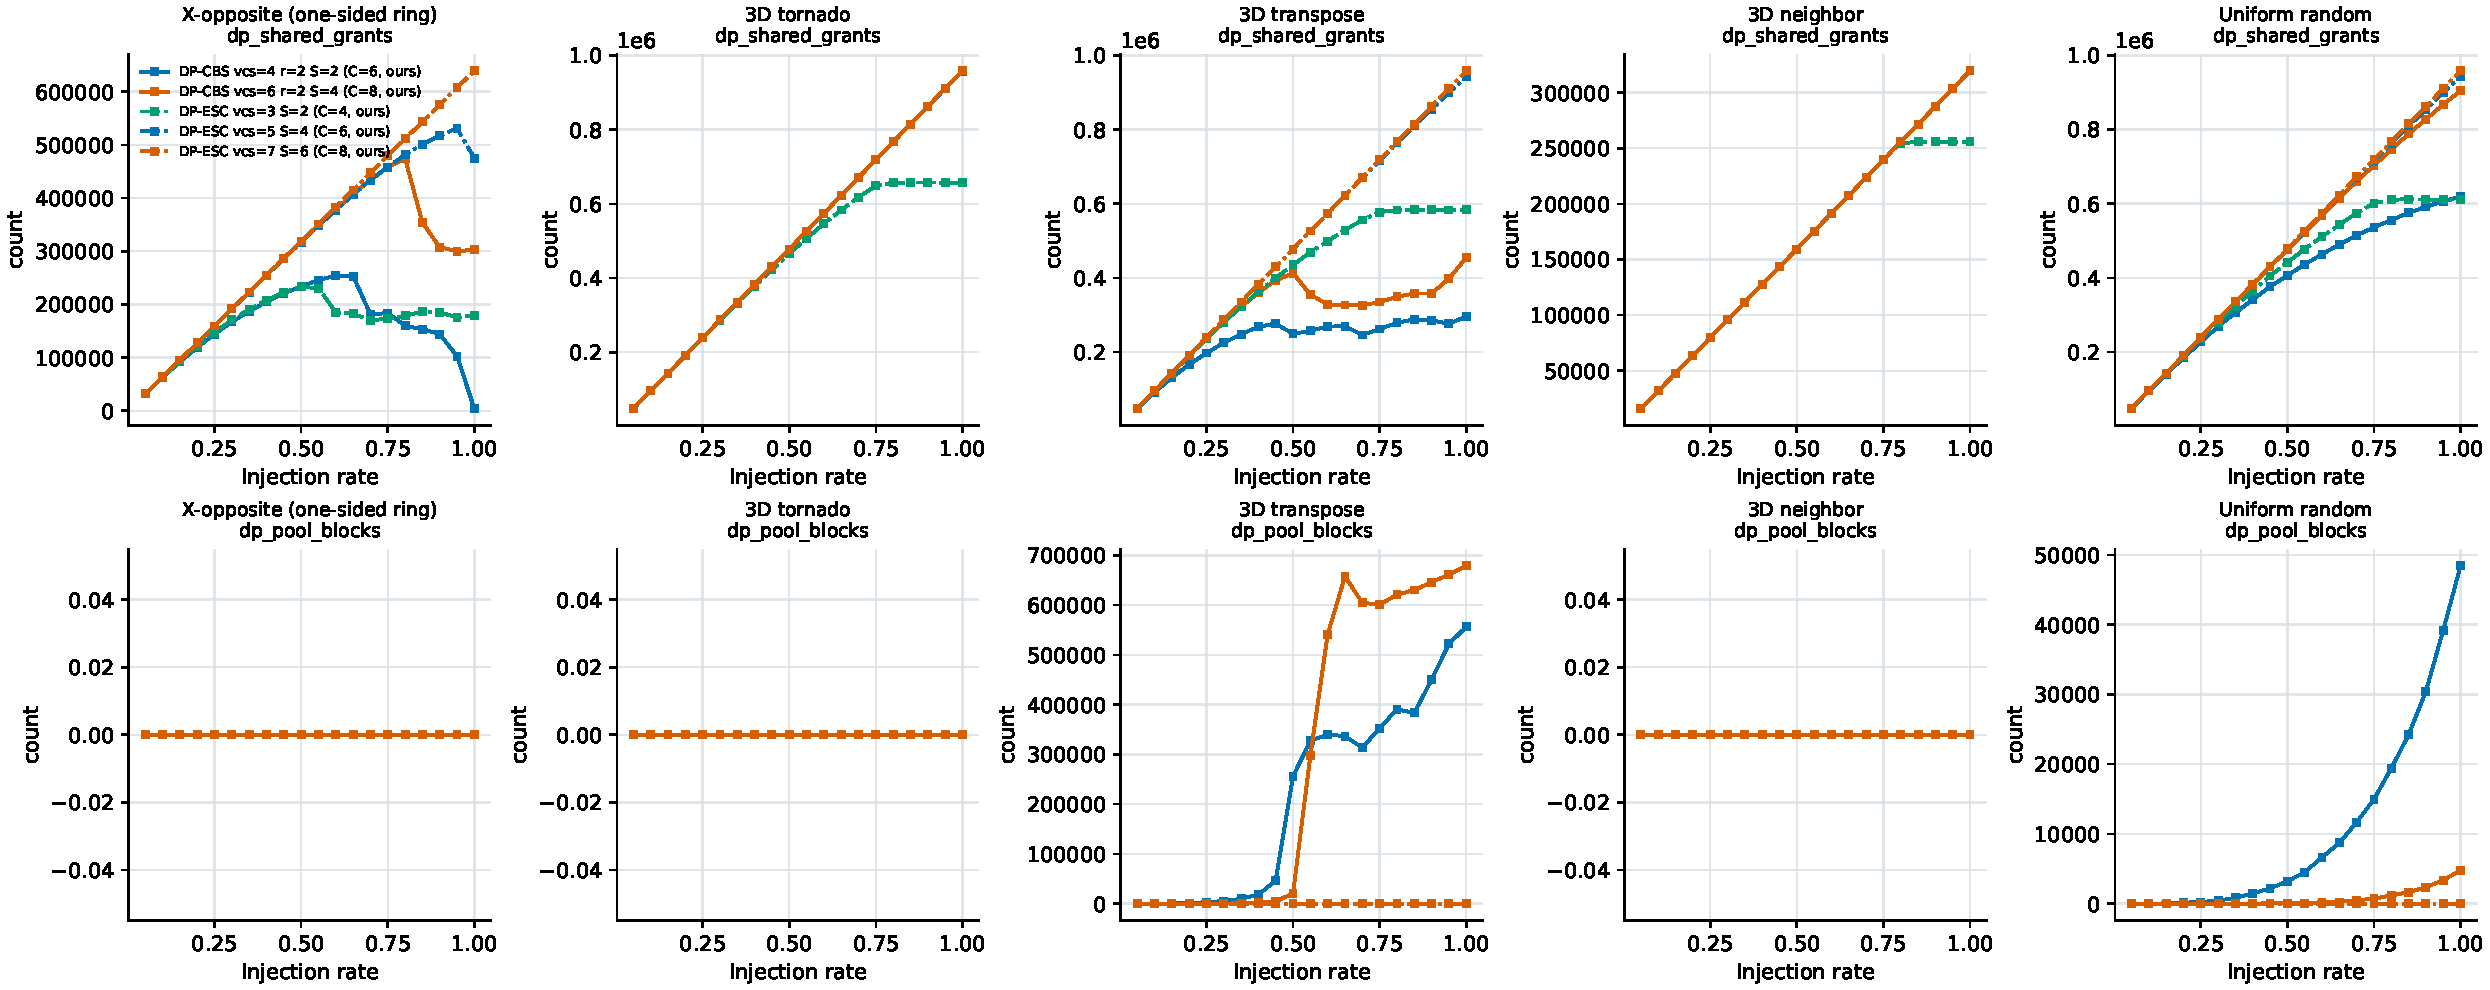
\includegraphics[width=\textwidth]{dp_activity}
  \caption{Pool activity vs.\ injection rate for the DP modes:
  \texttt{dp\_shared\_grants} (top row) and \texttt{dp\_pool\_blocks}
  (bottom row) per pattern.}
  \label{fig:activity}
\end{figure}

\section{Analysis}
\label{sec:analysis}

\subsection{Why pooling wins}

Three layers explain the gains:

\begin{enumerate}
  \item \textbf{Statistical multiplexing of buffer capacity.} Pooling
    converts private idle capacity into shared usable capacity; its value
    is exactly the demand imbalance between the two directions. This
    predicts the observed pattern dependence: adversarial one-sided
    patterns gain 20--31\%, symmetric uniform random gains $\approx$0.
  \item \textbf{The concrete bottleneck is hot-inport lane count
    $\times$ credit round trip.} On this substrate a VC holds one packet
    and turns around in $\sim$5 cycles, so each usable lane on the hot
    inport is worth $\approx$0.2 packets/cycle of saturation throughput.
    DP raises the number of lanes the hot direction may \emph{occupy}
    (dedicated + whole cap instead of dedicated + half the storage), a
    latency-hiding effect analogous to adding MSHRs to a cache. The
    family-B peak progression (reading 2, \S\ref{sec:experiments})
    matches this model quantitatively.
  \item \textbf{Separation of safety and performance resources.} What
    makes the first two layers \emph{safe to exploit} is that the pooled
    tranche carries no deadlock-freedom obligation: the substrate (CBS
    sub-ring or escape VCs) owns the invariants, so admission can fail
    arbitrarily. This separation is the design's transferable idea.
\end{enumerate}

\subsection{Costs and regime boundaries}

\textbf{Cap contention (reverse blocking).} Pooling's definitional cost:
under two-sided load, packets of one direction can exhaust the budget and
deny the other direction admission to its own physically free pooled VCs
($-32.6\%$ worst case at equal VC count). Three mitigations bound it: the
unpooled substrate guarantees a progress floor for the denied side,
DP-ESC reroutes around full pools at route-computation time, and
occupancy leaks back within a credit round trip ($\sim$5 cycles).
Per-side fairness under sustained asymmetry (aging, per-side floors
beyond the substrate) is left as future work.

\textbf{Buffer-rich regimes.} At $C{=}8$ every mechanism drowns in
buffers: DP-CBS turns slightly negative and family B saturates the
harness ceiling. DP targets scarce-buffer designs.

\textbf{State staleness.} The simulated registry is a zero-latency
oracle. A real sideband adds 1--2 cycles of skew; since the accounting
window already includes the credit round trip and is conservative, safety
is unaffected, and a token-conserved realization brackets the modeled
performance from below. The headline one-sided regimes are insensitive
(tokens park at the hot side); the marginal cells (+1--3\%) may erode
toward zero.

\textbf{Substrate specificity.} With one-flit control VCs, every extra
usable hot-side slot is worth a full $1/\text{RTT}$ of throughput; deeper
VCs would shrink the magnitudes (the direction of the effect stands).
Half of Table~\ref{tab:gains} (15/25 cells) sits at the injection ceiling
and says nothing about relative headroom; single-seed cells at $\pm$1--3\%
are reported as zero-cost bounds, not gains.

\section{Conclusion}

Dimension Pool shows that the static per-direction split of router
buffers is a real inefficiency on tori and that it can be removed with a
counter-only occupancy budget --- provided the deadlock-freedom invariant
lives in a resource the pool can never touch. Composed with CBS or with
escape VCs on a 4$\times$4$\times$4 Garnet Torus3D, DP delivers
+21--31\% (DP-ESC, $C{=}6$, all patterns) and +20.9\% (DP-CBS, $C{=}6$,
xopposite) peak stable throughput at equal usable storage, is neutral on
symmetric traffic, deadlock-free across 1006 runs, and comes with
explicitly mapped costs: cap contention under two-sided load, no benefit
in buffer-rich regimes, and a wiring sideband as the honest hardware
price.

\begin{thebibliography}{9}

\bibitem{dally1987}
W.~J. Dally and C.~L. Seitz,
``Deadlock-free message routing in multiprocessor interconnection
networks,''
\emph{IEEE Transactions on Computers}, vol.~C-36, no.~5, 1987.

\bibitem{dally1992}
W.~J. Dally,
``Virtual-channel flow control,''
\emph{IEEE Transactions on Parallel and Distributed Systems}, vol.~3,
no.~2, 1992.

\bibitem{duato1993}
J.~Duato,
``A new theory of deadlock-free adaptive routing in wormhole networks,''
\emph{IEEE Transactions on Parallel and Distributed Systems}, vol.~4,
no.~12, 1993.

\bibitem{chen2011}
L.~Chen, R.~Wang, and T.~M. Pinkston,
``Critical bubble scheme: An efficient implementation of globally aware
network flow control,''
in \emph{IEEE International Parallel \& Distributed Processing Symposium
(IPDPS)}, 2011.

\bibitem{dallytowles}
W.~J. Dally and B.~Towles,
\emph{Principles and Practices of Interconnection Networks}.
Morgan Kaufmann, 2004.

\end{thebibliography}

\end{document}
